\documentclass{standalone}
\usepackage{tikz}
\usepackage{ctex,siunitx}
\setCJKmainfont{Noto Serif CJK SC}
\usepackage{tkz-euclide}
\usepackage{amsmath}
\usepackage{wasysym}
\usetikzlibrary{patterns, calc}
\usetikzlibrary {decorations.pathmorphing, decorations.pathreplacing, decorations.shapes,}
\begin{document}
\small
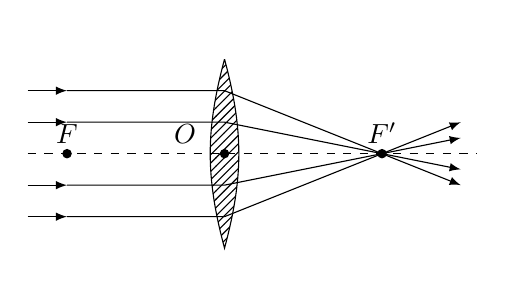
\begin{tikzpicture}[>=latex,scale=1.0]
  \useasboundingbox(-2.5,-1.6)rectangle(3.2,1.6);
  \draw [pattern=north east lines] (0,1.2) to [bend left=15] (0,-1.2) to [bend left=15](0,1.2);
  \draw [dashed] (-2.5,0)--(3.2,0);
  \draw (0,0)[fill=black] circle (1.5pt);
  \draw (-2,0)[fill=black] circle (1.5pt);    \draw (2,0)[fill=black] circle (1.5pt);
  \foreach \x in {-.8,-.4,.4,.8}
  {
      \draw[->] (-2.5,\x)--(-2,\x);
  }    
  \draw[->] (-2,-.8)--(0,-.8)--(2,0)--(3, .4)   ;
  \draw[->] (-2,-.4)--(0,-.4)--(2,0)--(3, .2)   ;
  \draw[->] (-2,.4)--(0,.4)--(2,0)--(3, -.2)   ;
  \draw[->] (-2,.8)--(0,.8)--(2,0)--(3, -.4)   ;
  \node at (-2,0)[above]{$F$};
  \node at (2,0)[above]{$F'$};
  \node at (-.5,0)[above]{$O$};
\end{tikzpicture}
\end{document}